%\chapter{Biologischer Hintergrund}\label{chap:biology}

%In diesem Kapitel wird beschrieben, in welchem Zusammenhang der Chlorophyllgehalt einer Pflanze mit der Vitalität eben dieser steht. Und es wird erklärt wie der Chlorophyllgehalt %genutzt werden kann, um  den Stresslevel einer Pflanze zu bestimmen.

\chapter{Konzept}\label{chap:concept}

\section{Normalized Difference Vegetation Index}\label{sec:ndvi}

Es gibt eine starke Korrelation zwischen dem physiologischen Status einer Pflanze und deren Chlorophyllgehalt. Faktoren wie Krankheit, Dürre oder Umweltverschmutzung haben einen negativen Einfluss auf den Chlorophyllspiegel.\cite{ref:hendry} Messungen haben ergeben, dass es einen Verbindung zwischen dem Reflexionsgrad im nahen Infrarotbereich und im Rotbereich und dem Chlorophyllgehalt gibt. Das heißt, dass eine gesunde, adulte Pflanze im nahen Infrarotbereich stärker reflektiert als zum Beispiel eine pathologisch veränderte Pflanze. Jedoch bleibt die Reflexion im roten Lichtspektrum in beiden Fällen vergleichsweise schwach. Andere vegetationsfreie Oberflächen wie Acker, Straßen oder Wasser strahlen auch im nahen Infrarotbereich schwach zurück. Dadurch ergibt sich eine zerstörungsfreie Methode, mit einer Multispektralkamera die Vitalität ("`Grünheit"') einer oder mehrerer Pflanzen zu bestimmen.\cite{ref:anatoly} \\\\
Eine multispektralen Aufnahme kann mithilfe der Formel 
\begin{equation}\label{equation:ndvi}
	NDVI = \frac{Band_{NIR} - Band_{Red}} {Band_{NIR} + Band_{Red}}
\end{equation}
dazu genutzt werden, den \textit{Normalized Difference Vegetation Index} (NDVI) zu berechnen. Wobei $Band_{NIR}$ der nahe Infrarotbereich (Near Infrared) und $Band_{RED}$ der sichtbare rote Bereich des elektromagnetischen Spektrums ist. Der NDVI gibt quantifizierte Werte im Bereich von $-1$ bis $1$ zurück. Dabei deuten Werte, die kleiner als $0$ sind, auf Wasserobflächen hin. $0$ bedeutet keine Vegetation. Bei Werte nahe $0$ handelt es sich um spärliche oder ungesunde Vegetation. Das bedeutet je näher ein Wert an $1$ ist, desto dichter bewachsen und gesünder ist die beobachtete Vegetationsfläche.\cite{ref:nasa} Dass bei einem niedrigen, positiven NDVI nicht unterschieden werden kann, ob eine Fläche kaum bewachsen ist oder ungesunde Vegetation besitzt, kann hier vernachlässigt werden. Das Gebiet, das in dieser Arbeit untersucht wird, ist ein bewachsenes Feld, so kann man geringe Vegetation ausschließen. 

\section{Sentinel-2}\label{sec:sentinel2}

Die Sentinel-2-Satelliten sind eine von sechs Satellitenarten (Sentinel-1 bis -6) des Copernicus-Programms\footnote{Das Copernicus-Programm wurde von der Europäischen Union zur Erdbeobachtung ins Leben gerufen. Die gesammelten Daten werden für wissenschaftliche, wirtschaftliche und private Anwendungszwecke zur Verfügung gestellt.\cite{ref:copernicus}}, die zur Erdbeobachtung in einen 786 km hohen sonnensynchronen Orbit gebracht wurden. Die Instrumente der Sentinel-2-Satelliten können Aufnahmen in Bereichen des roten und nahen Infrarot- bis hin zum Kurzwelleninfrarotspektrums. Die Aufnahmen haben Gesamtgröße von $100*100$ km und je nach Band eine von Auflösung von 10m, 20m oder 60m (s. Tabelle \ref{tab:resolutions}).

\begin{table}[ht]
\begin{tabular}{c|c|c|c}
Bandnummer & Räumliche Auflösung & Mittlere Wellenlänge (nm) & Bandbreite (nm) \\
\hline
B1 & 60 & 443,9 & 27\\
B2 & 10 & 496,6 & 98\\
B3 & 10 & 560 & 45\\
B4 & 10 & 664,5 & 38\\
B5 & 20 & 703,9 & 19\\
B6 & 20 & 740,2 & 18\\
B7 & 20 & 782,5 & 28\\
B8 & 10 & 835,1 & 145\\
B8a & 20 & 864,8 & 33\\
B9 & 60 & 945 & 26\\
B10 & 60 & 1373,5 & 75\\
B11 & 20 & 1613,7 & 143\\
B12 & 20 & 2202,4 & 242\\
\end{tabular}
\caption{Räumliche und spektrale Auflösungen von Sentinel-2A\cite{ref:sentinel:radiores}}\label{tab:resolutions}
\end{table}
\noindent
Besonders wichtig sind die Bänder B4 (Rot) und B8 (Nahes Infrarot). Mit diesen Bändern kann der NDVI (s. Kapitel \ref{sec:ndvi}) berechnet werden.\cite{ref:sentinel:ndvi} Die Sentinel-2-Satelliten bieten mit $10*10$ m pro Pixel eine hohe räumliche Auflösung.\footnote{Im Vergleich hat zum Beispiel der Landsat-8-Satellit, dessen Daten ebenfalls frei verfügbar sind, eine relativ geringe Auflösung von $30*30$ m.\cite{ref:landsat}} Diese Eigenschaft ist wichtig, um eine mögliche Infizierung genau eingrenzen zu können.\\\\
Dabei ist es auch wichtig, dass die Satelliten regelmäßige Daten liefern können. Durch die gemeinsame Konstellation übertragen die Plattformen alle fünf Tage Daten über einen spezifischen Punkt auf der Erdoberfläche.\cite{ref:sentinel:resolutions} Damit ist gewährleistet, dass der Feldbesitzer ohne persönliche Inspektion ein bis zweimal in der Woche eine Gesundheitseinschätzung über seine Felder erhält.

\section{Mask R-CNN}\label{sec:maskrcnn}
In Kapitel \ref{sec:ndvi} und \ref{sec:sentinel2} wurde erklärt wie Daten über die möglichen Erkrankungen geliefert und verarbeitet werden können. Auf den zugrunde liegenden Bilddaten soll nun ein künstliches neuronales Netzwerk (KNN) trainiert werden. In diesem Kapitel wird darauf eingegangen, welche Anforderungen an das KNN gestellt werden, warum das Titel gebende Netz ausgewählt wurde und wie dieses funktioniert.

\subsection{Anforderungen}\label{sec:sub:requirements}
Das KNN muss in der Lage sein, wahrscheinliche Krankheiten in der zu untersuchenden Agrarfläche möglichst genau eingrenzen und klassifizieren zu können. Das ist besonders wichtig, wenn ein Feld von multiplen Krankheiten betroffen ist.\\\\
Es ist damit zu rechnen, dass Daten unter bewölkten Bedingungen aufgenommen werden. Nach starken Niederschlägen können Acker teils oder gänzlich überflutet sein.\cite{ref:root-rot} Das sorgt selbst unter wolkenfreien Bedingungen für einen niedrigen NDVI, obwohl die Nutzpflanzen gesund sind. Das neuronale Netz muss mit solchen \glqq Ausreißern\grqq{} umgehen können.
\\\\
Daraus ergeben sich folgende Kriterien für das neuronale Netzwerk:

\begin{itemize}
	\item Erkennung auf Pixelebene
	\item Robustheit
	\item Hohe Genauigkeit 
\end{itemize}

\subsection{Grundlagen}\label{sec:sub:basics}

\subsubsection{Vollständig vernetztes neuronales Netz}

\noindent
Künstliche neuronale Netze sind nach dem Vorbild von biologischen neuronalen Netzen gebildet worden. So ist ein KNN ebenfalls eine Verbindung von künstlichen Neuronen. Diese Neuronen sind in Schichten angeordnet und jede die Neuronen einer Schicht sind mit den Neuronen nächsten bzw. letzten Schicht verbunden. Zwischen der ersten und der letzten sog. Ausgangsschicht existieren $n$ versteckte Schichten (engl.: hidden layers). 

\begin{figure}[ht]
  \centering
  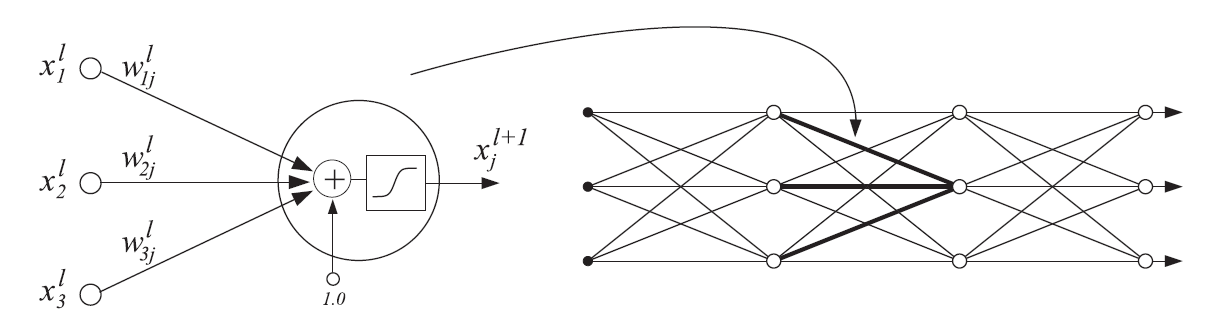
\includegraphics[width=0.8\textwidth]{pics/neural-net.PNG}
  \caption[Künstliches neuronales Netz]{Künstliches neuronales Netz\cite{ref:verrelst}}
  \label{fig:ann}
\end{figure}
\noindent
Ein Neuron besitzt mehrere Eingangsverbindungen (Gewichte) und ein Ausgangsneuron. Ob ein Neuron "`feuert"', wird durch eine lineare oder nicht-lineare Aktivierungsfunktion bestimmt. Die Eingangsgewichte sind veränderbare Werte, die je nach Höhe einen starken oder niedrigen Einfluss auf die Aktivierungsfunktion haben.
\begin{equation}\label{equ:neuron}
x^{l+1}_{j}=f(\sum\nolimits_i w^l_{ij}x^l_i + w^l_{bj})
\end{equation}
beschreibt das Neuron $j$ in Schicht $l+1$, wobei
\begin{itemize}
	\item $w^l_{ij}$ die Gewichte sind, die Neuron $i$ in Schicht $l$ mit Neuron $j$ verbinden.
	\item $w^l_{bj}$ der Biasterm des $j$-ten Neurons in Schicht $l$ ist.
	\item $f$ die Aktivierungsfunktion ist.\cite{ref:verrelst}
\end{itemize} 

\subsubsection{Convolutional Neural Networks}\label{sec:sub:sub:cnn}
\begin{figure}[ht]
  \centering
  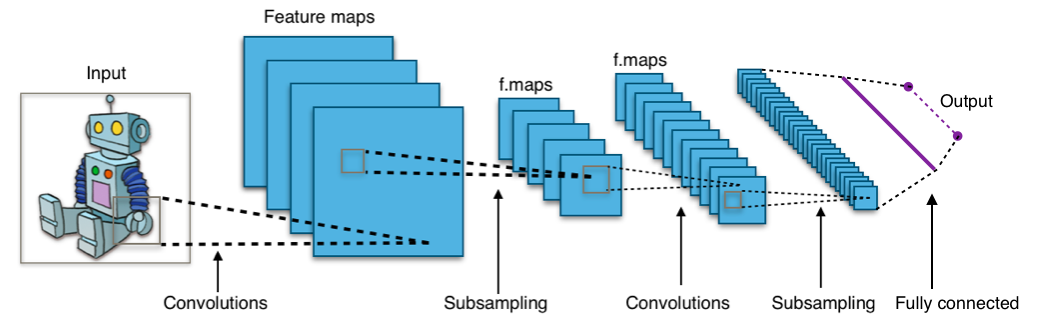
\includegraphics[width=0.95\textwidth]{pics/cnn.png}
  \caption[CNN]{Architektur eines Convolutional Neural Network\cite{ref:cnn-architecture}}
  \label{fig:cnn-architecture}
\end{figure}

\noindent 
\textit{Convolutional Neural Networks} (CNN, dt.: faltendes neuronales Netzwerk) sind Kategorien von neuronalen Netzen, die besonders in der \textit{Computer Vision} Anwendung finden. In der ersten Schicht werden mehrere Merkmale (engl.: features) durch Filter extrahiert und in separate sog. \textit{Feature Maps} abgelegt, um größere Abstraktionsebenen zu erreichen. Diese Filter sind mathematisch mit Faltungen (engl.: convolutions) zu vergleichen und geben dem Netz den Namen. 
\\\\
Die Dimensionen der Feature Maps werden in einem Poolingschritt\footnote{Es gibt verschiedene Arten von Pooling (Max, Average, Sum, ...). Dabei wird die $m*m$ px große Feature Map in sich angrenzende $n*n$ px große Felder eingeteilt ($n<m$). Im Falle von Max-Pooling wird der höchste Wert aus dem Feld übernommen.} (oder auch \textit{subsampling}) reduziert. Dadurch bleiben nur relevante Informationen erhalten und das CNN wird bis zu einem gewissen Grad robust gegenüber Translationen und Rotationen. In der Regel werden die Faltungen und das das Pooling zwei Mal durchgeführt, wie es in Abb. \ref{fig:cnn-architecture} abgebildet ist.
\\\\
Nach der Merkmalextraktion werden die Feature Maps zur Klassifikation in eine eindimensionale Schichten geglättet. Die folgenden Schichten bis zur Ausgangsschicht sind vollständig vernetzt.


\subsection{Mask R-CNN}\label{sec:sub:mask-rcnn}

Im Rahmen dieser Arbeit wird das \textit{Mask Region-based Convolutional Neural Network} untersucht. Mask R-CNN ist eine von Facebook AI Research (FAIR) entwickelte Erweiterung des \textit{Faster R-CNN} und kann verschiedene Instanzen einer Klasse in einem Bild von einander trennen. Dazu muss zuerst die Begriffe der Instanzsegmentierung definiert werden.
\\\\
\begin{figure}[ht]
  \centering
  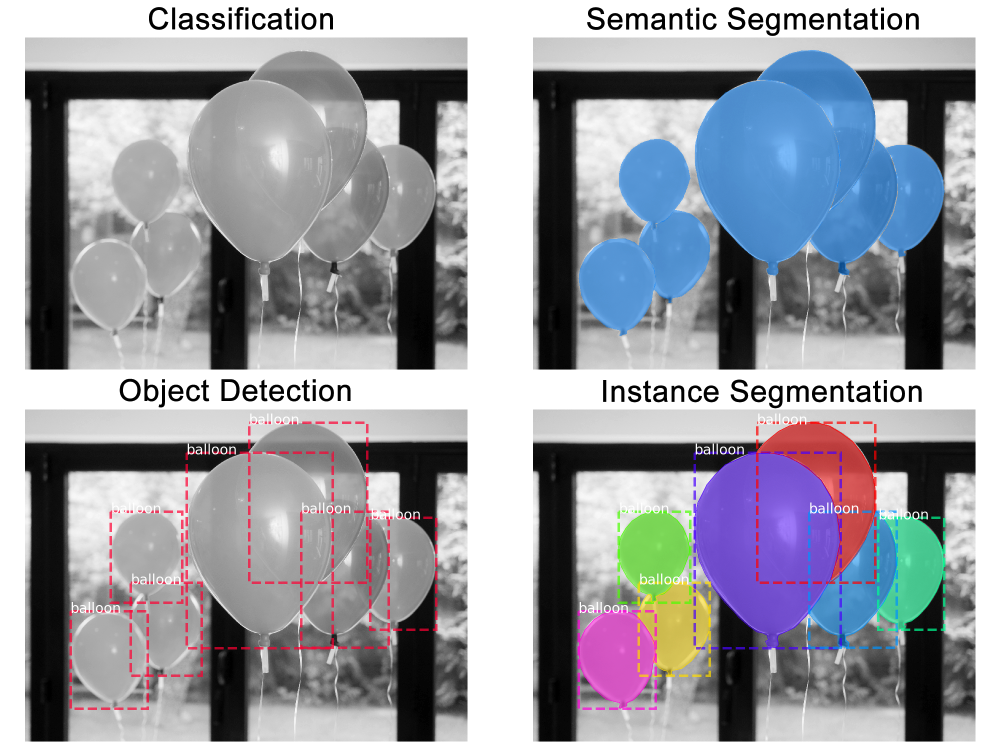
\includegraphics[width=0.8\textwidth]{pics/instance-segmentation.png}
  \caption[Instanzsegmentierung]{Unterschied Klassifizierung / semantische Segmentierung / Objekterkennung / Instanzsegmentierung\cite{ref:matterport:maskrcnn}}
  \label{fig:instance-segmentation}
\end{figure}
\noindent
Einfache Klassifizierung (engl.: classification) ordnet Bilder als Ganzes einer Klasse zu. \textit{Semantische Segmentierung} (engl.: semantic segmentation) beschreibt die Klassifizierung auf Pixelebene. Es wird erkannt zu welcher Klasse eine Menge von Pixeln gehören, aber es wird nicht zwischen einzelnen Objekten unterschieden. \textit{Objekterkennung} (engl.: object detection) entdeckt und lokalisiert unterschiedliche Objekte, indem es eine Bounding Box um jedes erkannte Objekt zieht. Jedoch fehlt hier die pixelgenaue Abgrenzung einzelner Objektinstanzen. \text{Instanzsegmentierung} (engl.: instance segmentation) kombiniert \textit{Objekterkennung} und \textit{semantische Segmentierung} und ist so in der Lage zwischen einzelnen Objekten zu unterscheiden und ihnen entsprechende Pixel zuzuordnen (s. Abb. \ref{fig:instance-segmentation}) und ist eine der größten Herausforderungen in der Bildverarbeitung.\cite{ref:maskrcnn}
\\\\
\begin{figure}[ht]
  \centering
  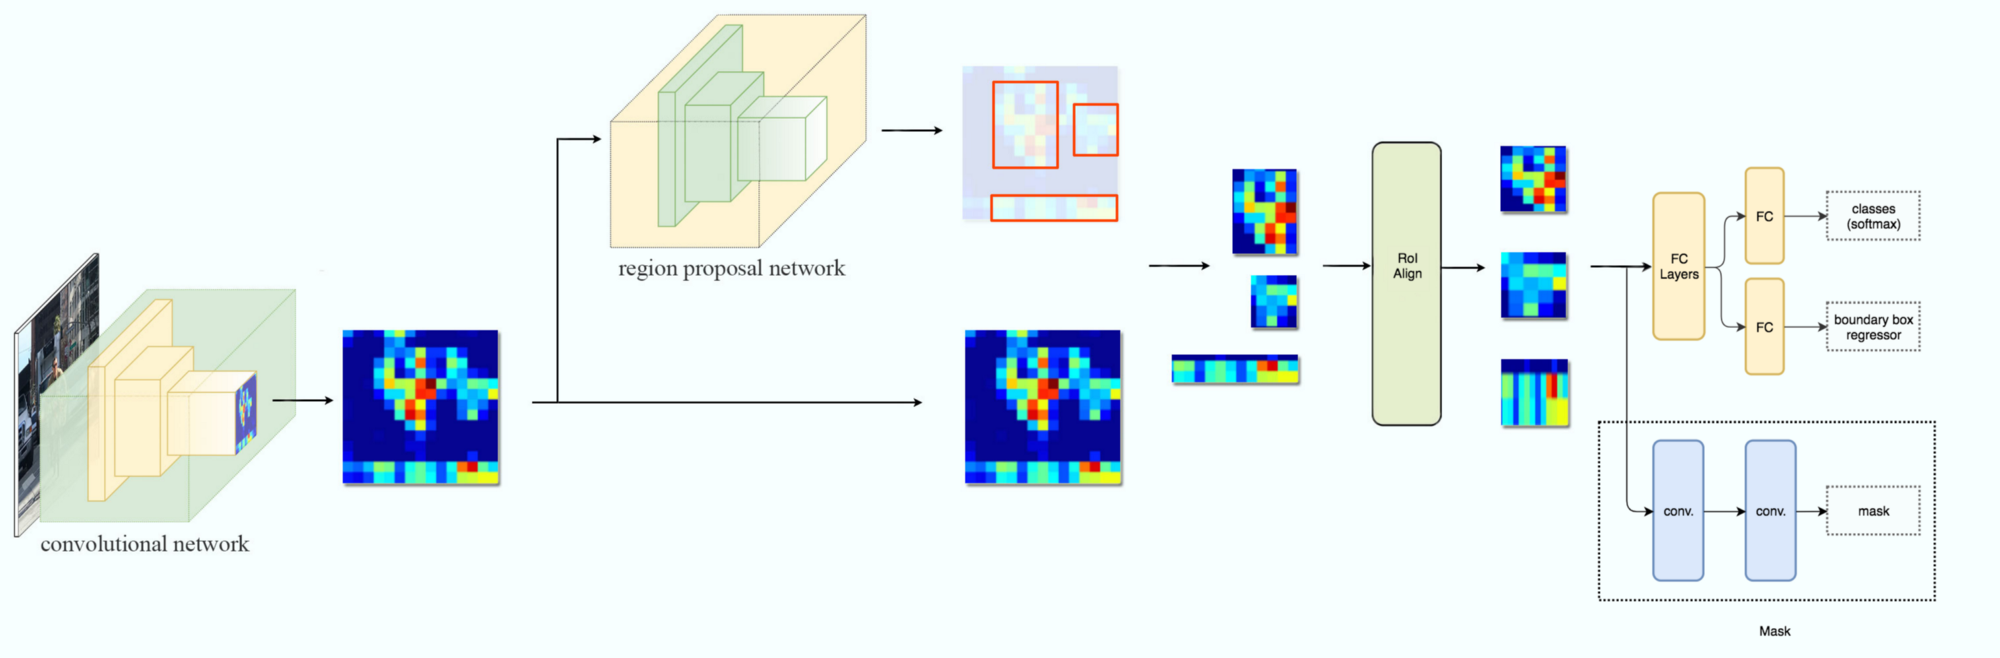
\includegraphics[width=\textwidth]{pics/maskrcnn-archtecture.PNG}
  \caption[Mask R-CNN-Architektur]{Mask R-CNN-Architektur\cite{ref:mask-rcnn-architecture}}
  \label{fig:maskrcnn-architecture}
\end{figure}

\noindent
Mask R-CNN ist wie Faster R-CNN in zwei Segmente eingeteilt. In dem ersten Segment, dem \textit{Region Proposal Network} (RPN, dt.: Region vorschlagendes Netzwerk), werden mehrere Rahmen (Bounding Boxes) innerhalb eines Bildes vorgeschlagen, die interessante Objekte beinhalten könnten.\cite{ref:faster-r-cnn} Die vorgeschlagene Regionen, die einzeln von CNNs bewertet werden, ist der Kernansatz von R-CNN. Das RPN wurde identisch von Faster R-CNN für Mask R-CNN übernommen.\cite{ref:maskrcnn} 
\\\\
Im zweiten Segment werden aus den Regionen \textit{Bounding Boxes} (dt.: Rahmen) und Masken generiert und klassifiziert. Die Rahmen haben verschiedene Größen und können Probleme bei der Klassifizierung verursachen. Daher werden die Rahmen auf eine kleine Feature Map gleicher Größe (z.B. $7*7$ px) reduziert. Die Authoren von \cite{ref:maskrcnn} schlagen eine Methode namens \textit{RoI-Align} vor, bei der Proben aus der Feature Map entnommen werden und eine bilineare Interpolation angewendet wird. In dem bei Faster R-CNN angewandten Verfahren \textit{RoI-Pooling} entstehen durch Quantisierung Informationsverluste und räumliche Abweichungen zwischen Bounding Box und Feature Map, was negative Auswirkungen auf die Maskengenerierung haben kann.\cite{ref:maskrcnn}
\\\\
%\begin{figure}[ht]
%  \centering
%  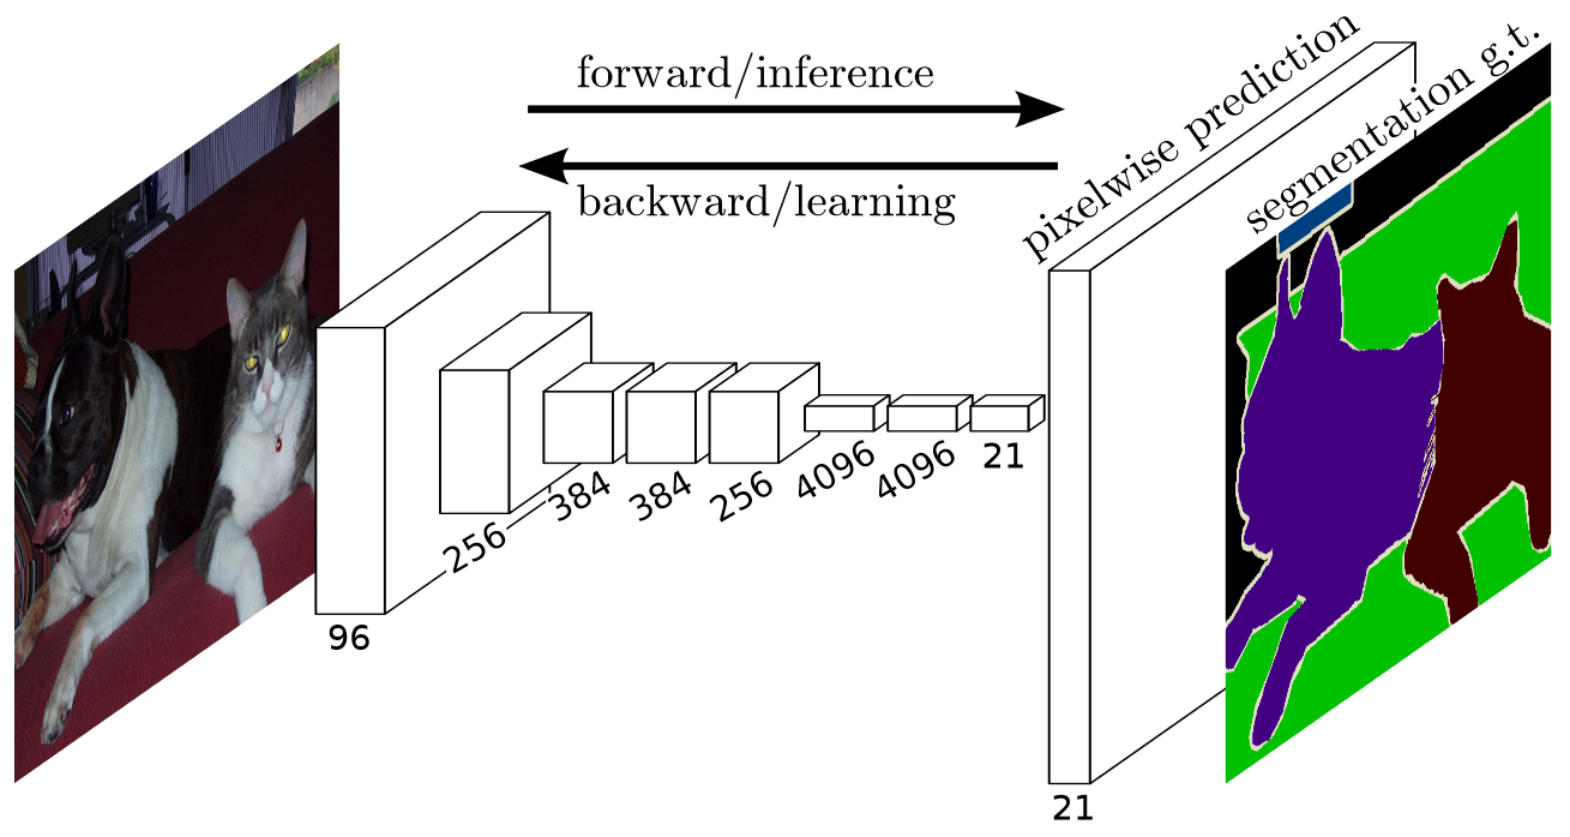
\includegraphics[width=0.90\textwidth]{pics/fcn-architecture.PNG}
%  \caption[FCN-Architektur]{FCN-Architektur\cite{ref:mask-rcnn-architecture}}
%  \label{fig:fcn-architecture}
%\end{figure}
%\noindent
Die oberen vollständig vernetzten Schichten (\textit{FC Layers} in Abb. \ref{fig:maskrcnn-architecture}) klassifizieren die Regionen und die Bounding Boxes berechnet. Dieser Zweig ist für die Objekterkennung wichtig und noch mit Faster R-CNN gemeinsam. 
\\\\
Gleichzeitig werden in einem parallelen Zweig je Bounding Box $k$ $m*n$ große Masken zur semantischen Segmentierung erzeugt, wobei $k$ die Anzahl der Klassen ist.  Anders als in dem ersten Zweig des zweiten Segmentes werden die Masken durch \textit{fully convolutional networks} (FCN, dt.: vollständig faltende Netzwerke) prognostiziert. Diese bestehen nur aus faltenden Schichten, wie sie in Kapitel \ref{sec:sub:sub:cnn} beschrieben sind. Eine Maske ist eine räumliche Kodierung eines Objektes und daher ist es wichtig räumliche Informationen beizubehalten. Diese können durch die Pixel-zu-Pixel-Übereinstimmung extrahiert werden, welche sonst durch vollständig vernetzter Schichten verloren gehen. Diese geben einen Vektor ohne räumliche Dimensionen aus.\cite{ref:maskrcnn} \todo{FCN und wie wird Maske erzeugt?}
\\\\
\begin{figure}[ht]
  \centering
  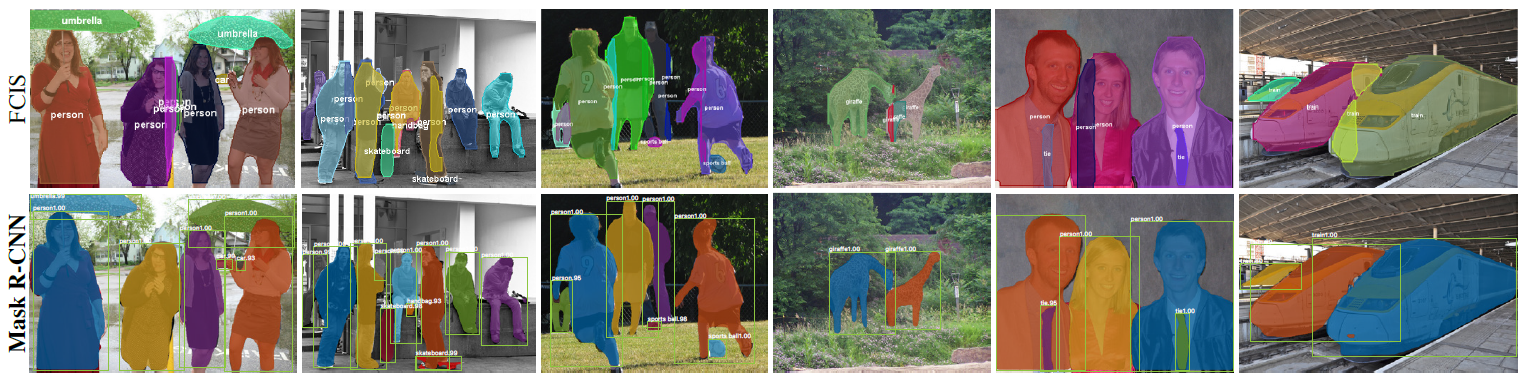
\includegraphics[width=\textwidth, height=5cm]{pics/mrcnn-vs-fcis.PNG}
  \caption[Mask R-CNN vs. FCIS]{Bei FCIS entstehen Artefakte, wenn Objekte sich in einem Bild überlappen.\cite{ref:maskrcnn}}
  \label{fig:maskvsfcis}
\end{figure}
\begin{table}[ht]
  \centering
  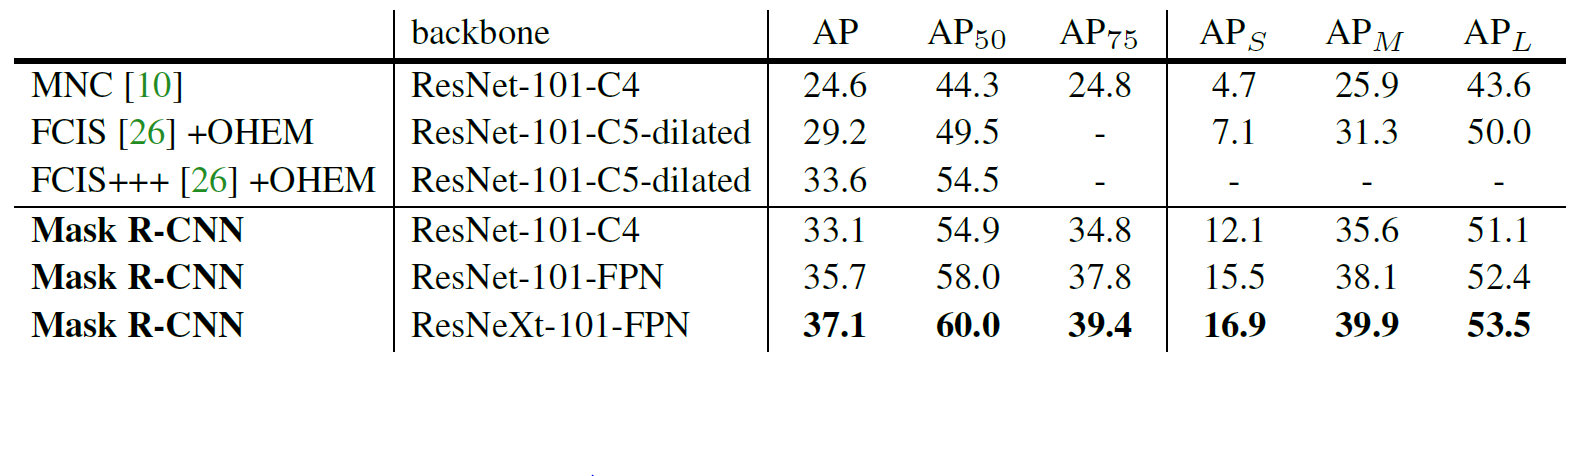
\includegraphics[width=\textwidth]{pics/mrcnn-vs-fcis-vs-mnc.PNG}
  \caption[Mask R-CNN im Vergleich]{Instance segmentation \textit{mask} AP auf COCO \textit{test-dev}. MNC und FCIS sind Sieger der COCO 2015 und 2016 Challenge. Mask R-CNN erzielt deutlich bessere Ergebnisse als die komplexere FCIS+++.\cite{ref:maskrcnn}}
  \label{tab:maskvsfcisvsmnc}
\end{table}
\noindent
In \cite{ref:maskrcnn} wird Mask R-CNN mit den \textit{COCO challenge}-Gewinnern\footnote{COCO (Common Objects in Context, dt.: Gewöhnliche Objekte im Kontext) enthält einen Datensatz von über 200000 Bildern in über 80 Kategorien. Der Datensatz ist eine oft genutzte Basis, um Objekterkennungstechniken zu evaluieren und zu bewerten.\cite{ref:coco}} der Jahre 2015 und 2016 verglichen. Der Vergleich zeigt, dass Mask R-CNN in der Challenge bessere Werte erzielt als die Konkurenten (s. Tab. \. Desweiteren fällt \textit{fully convolutional instance segmentation} (FCIS, dt.: vollständig faltende Instanzsegmentierung) auf, wenn es mit überlappenden Objekten konfrontiert wird. Dort erzeugt es Artefakte, welche durch Mask R-CNN nicht entstehen (s. Abb. \ref{fig:maskvsfcis}). Durch diese Gegenüberstellungen wird gezeigt, dass Mask R-CNN alle aufgeführten Anforderungen erzielt. Es erkennt Klasseninstanzen auf Pixelebene und weist eine hohe Robustheit auf. Auch die Genauigkeit hebt sich beim direkten Vergleich ab. Aus diesen Gründen wurde Mask R-CNN im Rahmen diese Arbeit ausgewählt.

\subsection{Implementa}